\documentclass[12pt,a4paper,oneside]{report}

\usepackage[margin=1in]{geometry}
\usepackage[T1]{fontenc}
\usepackage[utf8]{inputenc}
\usepackage{newtxtext,newtxmath}
\usepackage{setspace}
\usepackage{graphicx}
\usepackage{array}
\usepackage{booktabs}
\usepackage{longtable}
\usepackage{tabularx}
\usepackage{multirow}
\usepackage{enumitem}
\usepackage{caption}
\usepackage{subcaption}
\usepackage{float}
\usepackage{pdflscape}
\usepackage{xcolor}
\usepackage{tikz}
\usetikzlibrary{arrows.meta,positioning,shapes.geometric,shapes.misc,fit,calc,decorations.pathmorphing}
\usepackage[hidelinks]{hyperref}
\usepackage{titlesec}

\onehalfspacing
\setlength{\parindent}{0pt}
\setlength{\parskip}{6pt}
\renewcommand{\arraystretch}{1.25}
\captionsetup{font=small,labelfont=bf}
\setlist[itemize]{leftmargin=*,topsep=2pt,itemsep=2pt}
\setlist[enumerate]{leftmargin=*,topsep=2pt,itemsep=2pt}

\definecolor{gvblue}{RGB}{9,32,63}
\definecolor{gvgreen}{RGB}{24,145,92}
\definecolor{gvcyan}{RGB}{27,116,158}
\definecolor{gvgray}{RGB}{246,248,250}
\definecolor{gvred}{RGB}{180,70,70}
\definecolor{gvyellow}{RGB}{247,184,75}

\tikzset{
  block/.style={rectangle, rounded corners=2pt, draw=gvblue, very thick, align=center, fill=gvgray, minimum height=9mm, text width=34mm, font=\small},
  wideblock/.style={rectangle, rounded corners=2pt, draw=gvblue, very thick, align=center, fill=gvgray, minimum height=9mm, text width=48mm, font=\small},
  smallblock/.style={rectangle, rounded corners=2pt, draw=gvblue, thick, align=center, fill=white, minimum height=7mm, text width=26mm, font=\scriptsize},
  decision/.style={diamond, draw=gvcyan, very thick, align=center, aspect=2.0, fill=blue!4, text width=27mm, font=\scriptsize},
  datastore/.style={cylinder, shape border rotate=90, draw=gvgreen, very thick, fill=green!5, aspect=0.28, align=center, minimum height=10mm, text width=31mm, font=\small},
  actor/.style={circle, draw=gvblue, very thick, fill=white, align=center, minimum size=10mm, font=\small},
  arrow/.style={-{Latex[length=2.4mm]}, very thick, draw=gvblue},
  dashedarrow/.style={-{Latex[length=2.4mm]}, thick, dashed, draw=gvcyan},
  line/.style={very thick, draw=gvblue},
  lifeline/.style={dashed, draw=black!45},
  note/.style={rectangle, draw=gvyellow!80!black, fill=yellow!10, rounded corners=2pt, align=left, font=\scriptsize, text width=42mm}
}

\newcommand{\code}[1]{\texttt{#1}}

\newcommand{\flowfive}[6]{%
\begin{figure}[H]\centering
\resizebox{0.98\textwidth}{!}{%
\begin{tikzpicture}[node distance=15mm]
\node[block] (a) {#2};
\node[block, right=of a] (b) {#3};
\node[block, right=of b] (c) {#4};
\node[block, right=of c] (d) {#5};
\node[block, right=of d] (e) {#6};
\draw[arrow] (a) -- (b);
\draw[arrow] (b) -- (c);
\draw[arrow] (c) -- (d);
\draw[arrow] (d) -- (e);
\end{tikzpicture}}
\caption{#1}\end{figure}}

\newcommand{\dfdfour}[6]{%
\begin{figure}[H]\centering
\resizebox{0.95\textwidth}{!}{%
\begin{tikzpicture}[node distance=17mm]
\node[actor] (u) {#2};
\node[wideblock, right=of u] (p1) {#3};
\node[wideblock, right=of p1] (p2) {#4};
\node[datastore, below=14mm of p1] (d1) {#5};
\node[datastore, below=14mm of p2] (d2) {#6};
\draw[arrow] (u) -- node[above,font=\scriptsize]{request} (p1);
\draw[arrow] (p1) -- node[above,font=\scriptsize]{validated data} (p2);
\draw[arrow] (p1) -- (d1);
\draw[arrow] (p2) -- (d2);
\draw[arrow] (p2) to[bend left=16] node[above,font=\scriptsize]{response} (u);
\end{tikzpicture}}
\caption{#1}\end{figure}}

\newcommand{\statefive}[6]{%
\begin{figure}[H]\centering
\resizebox{0.90\textwidth}{!}{%
\begin{tikzpicture}[node distance=15mm]
\node[block] (s1) {#2};
\node[block, right=of s1] (s2) {#3};
\node[block, right=of s2] (s3) {#4};
\node[block, below=of s3] (s4) {#5};
\node[block, left=of s4] (s5) {#6};
\draw[arrow] (s1) -- (s2);
\draw[arrow] (s2) -- (s3);
\draw[arrow] (s3) -- (s4);
\draw[arrow] (s4) -- (s5);
\draw[arrow] (s5) to[bend left=30] (s2);
\end{tikzpicture}}
\caption{#1}\end{figure}}

\newcommand{\sequencefour}[7]{%
\begin{figure}[H]\centering
\resizebox{0.98\textwidth}{!}{%
\begin{tikzpicture}[x=1cm,y=1cm]
\node[smallblock] (a) at (0,0) {#2};
\node[smallblock] (b) at (4,0) {#3};
\node[smallblock] (c) at (8,0) {#4};
\node[smallblock] (d) at (12,0) {#5};
\draw[lifeline] (a.south) -- (0,-6.8);
\draw[lifeline] (b.south) -- (4,-6.8);
\draw[lifeline] (c.south) -- (8,-6.8);
\draw[lifeline] (d.south) -- (12,-6.8);
\draw[arrow] (0,-1.0) -- node[above,font=\scriptsize]{#6} (4,-1.0);
\draw[arrow] (4,-2.0) -- node[above,font=\scriptsize]{validate and call} (8,-2.0);
\draw[arrow] (8,-3.0) -- node[above,font=\scriptsize]{read/write} (12,-3.0);
\draw[arrow] (12,-4.0) -- node[above,font=\scriptsize]{result} (8,-4.0);
\draw[arrow] (8,-5.0) -- node[above,font=\scriptsize]{structured response} (4,-5.0);
\draw[arrow] (4,-6.0) -- node[above,font=\scriptsize]{#7} (0,-6.0);
\end{tikzpicture}}
\caption{#1}\end{figure}}

\newcommand{\componentfour}[5]{%
\begin{figure}[H]\centering
\resizebox{0.90\textwidth}{!}{%
\begin{tikzpicture}[node distance=12mm]
\node[wideblock] (a) {#2};
\node[wideblock, right=of a] (b) {#3};
\node[wideblock, right=of b] (c) {#4};
\node[wideblock, below=of b] (d) {#5};
\draw[arrow] (a) -- (b);
\draw[arrow] (b) -- (c);
\draw[arrow] (b) -- (d);
\draw[arrow] (c) -- (d);
\end{tikzpicture}}
\caption{#1}\end{figure}}

\newcommand{\layerdiagram}[6]{%
\begin{figure}[H]\centering
\resizebox{0.70\textwidth}{!}{%
\begin{tikzpicture}[node distance=6mm]
\node[wideblock, fill=blue!6] (l1) {#2};
\node[wideblock, below=of l1, fill=cyan!5] (l2) {#3};
\node[wideblock, below=of l2, fill=green!5] (l3) {#4};
\node[wideblock, below=of l3, fill=yellow!10] (l4) {#5};
\node[wideblock, below=of l4, fill=red!5] (l5) {#6};
\draw[arrow] (l1) -- (l2);
\draw[arrow] (l2) -- (l3);
\draw[arrow] (l3) -- (l4);
\draw[arrow] (l4) -- (l5);
\end{tikzpicture}}
\caption{Layer diagram}\end{figure}}

\newcommand{\structurechart}[6]{%
\begin{figure}[H]\centering
\resizebox{0.92\textwidth}{!}{%
\begin{tikzpicture}[node distance=10mm]
\node[wideblock] (root) {#2};
\node[smallblock, below left=14mm and 18mm of root] (a) {#3};
\node[smallblock, below=14mm of root] (b) {#4};
\node[smallblock, below right=14mm and 18mm of root] (c) {#5};
\node[smallblock, below=16mm of b] (d) {#6};
\draw[arrow] (root) -- (a);
\draw[arrow] (root) -- (b);
\draw[arrow] (root) -- (c);
\draw[arrow] (b) -- (d);
\end{tikzpicture}}
\caption{Structure chart}\end{figure}}

\newcommand{\interactionoverview}[6]{%
\begin{figure}[H]\centering
\resizebox{0.90\textwidth}{!}{%
\begin{tikzpicture}[node distance=10mm]
\node[block] (start) {Start};
\node[block, right=of start] (a) {#2};
\node[decision, right=of a] (b) {#3};
\node[block, above right=12mm and 14mm of b] (c) {#4};
\node[block, below right=12mm and 14mm of b] (d) {#5};
\node[block, right=34mm of b] (e) {#6};
\draw[arrow] (start) -- (a);
\draw[arrow] (a) -- (b);
\draw[arrow] (b) -- node[above,font=\scriptsize]{yes} (c);
\draw[arrow] (b) -- node[below,font=\scriptsize]{no/fallback} (d);
\draw[arrow] (c) -- (e);
\draw[arrow] (d) -- (e);
\end{tikzpicture}}
\caption{Interaction overview diagram}\end{figure}}

\begin{document}

\begin{titlepage}
\centering
\vspace*{0.5cm}
{\Large\bfseries GeoVision: AI-Powered GIS Platform for Intelligent Land-Use Planning and Environmental Risk Assessment\par}
\vspace{0.7cm}
\includegraphics[width=4cm]{../GeoVision_Final_LaTeX_Project/geovision_final_latex/ThesisFigs/FASTLogo.jpg}
\vspace{0.6cm}

{\large Project Team\par}
\vspace{0.3cm}
{\large Syed Muhammad Rehan \quad 22P-9145\par}
{\large Muhammad Taha Nafis \quad 22P-9299\par}
{\large Yousaf Maaz \quad 22P-9349\par}
\vspace{0.5cm}
{\large Session 2022-2026\par}
\vspace{0.8cm}
{\large Supervised by\par}
{\large Mr. Fazl-e-Basit\par}
\vspace{0.2cm}
{\large Co-Supervised by\par}
{\large Ms. Sara Rehmat\par}
\vspace{0.8cm}
{\large Department of Computer Science\par}
{\large National University of Computer and Emerging Sciences\par}
{\large Peshawar, Pakistan\par}
\vspace{0.4cm}
{\large June, 2026\par}
\end{titlepage}

\pagenumbering{roman}

\chapter*{Student's Declaration}
\begin{center}
\includegraphics[width=3cm]{../GeoVision_Final_LaTeX_Project/geovision_final_latex/ThesisFigs/FASTLogo.jpg}
\end{center}
\vspace{0.3cm}

We declare that this project titled ``GeoVision: AI-Powered GIS Platform for Intelligent Land-Use Planning and Environmental Risk Assessment'', submitted as a requirement for the award of the degree of Bachelors in Software Engineering, does not contain any material previously submitted for a degree in any university; and that to the best of our knowledge, it does not contain any materials previously published or written by another person except where due reference is made in the text.

We understand that the management of the Department of Computer Science, National University of Computer and Emerging Sciences, has a zero tolerance policy towards plagiarism. Therefore, we, as authors of the above-mentioned thesis, solemnly declare that no portion of our thesis has been plagiarized and any material used in this thesis from other sources is properly referenced.

We further understand that if we are found guilty of any form of plagiarism in the thesis work even after graduation, the University reserves the right to revoke our BS degree.

\vspace{1cm}
\begin{tabular}{p{0.55\textwidth}p{0.35\textwidth}}
Syed Muhammad Rehan & Signature: \\[0.6cm]
Muhammad Taha Nafis & Signature: \\[0.6cm]
Yousaf Maaz & Signature: \\[0.8cm]
Verified by Plagiarism Cell Officer & Dated:
\end{tabular}

\chapter*{Certificate of Approval}
The Department of Computer Science, National University of Computer and Emerging Sciences, accepts this thesis titled ``GeoVision: AI-Powered GIS Platform for Intelligent Land-Use Planning and Environmental Risk Assessment'', submitted by Syed Muhammad Rehan (22P-9145), Muhammad Taha Nafis (22P-9299), and Yousaf Maaz (22P-9349), in its current form, and it satisfies the dissertation requirements for the award of Bachelors Degree in Software Engineering.

\vspace{0.8cm}
\begin{tabular}{p{0.55\textwidth}p{0.35\textwidth}}
Supervisor: Mr. Fazl-e-Basit & Signature: \\[0.7cm]
Co-Supervisor: Ms. Sara Rehmat & Signature: \\[0.7cm]
Riaz Nawab & FYP Coordinator \\[0.7cm]
Dr. Qasim Jaan & HoD of Department of Computer Science
\end{tabular}

\chapter*{Acknowledgements}
We would like to express our sincere gratitude to our supervisor, Mr. Fazl-e-Basit, for his guidance, feedback, and encouragement throughout the development of GeoVision. We are also grateful to the Department of Computer Science at FAST-NUCES Peshawar for providing an academic environment in which this project could be designed, implemented, tested, and documented.

We thank our families and friends for their constant support during the final-year project cycle. We also acknowledge the open-source communities behind FastAPI, React, PostgreSQL, Redis, Leaflet, Deck.gl, and the geospatial and machine-learning libraries used in the project.

\vspace{0.8cm}
Syed Muhammad Rehan\\
Muhammad Taha Nafis\\
Yousaf Maaz

\chapter*{Abstract}
GeoVision is an AI-powered GIS decision-support platform designed to help urban planners inspect parcels, review environmental risk, query zoning information, generate alternative land-use plans, and preserve planning outputs for later review. Conventional early-stage land-use planning often requires switching between map tools, spreadsheets, regulatory documents, and manual scenario sketches. This fragmentation slows analysis and makes it difficult to explain why a parcel is recommended for a particular use.

The implemented project uses a React and TypeScript frontend with a FastAPI backend. The backend provides authentication, PostgreSQL-backed persistence, spatial optimization, zoning retrieval-augmented generation, planner copilot streaming, rule-based risk explanation, Redis-backed optimization caching, and saved map management. The frontend includes a protected workbench, environmental analysis workspace, layers and zoning page, plan gallery, saved plans interface, assignment explanation panel, settings page, and browser-generated planner PDF export.

This report follows the required FYP documentation structure. It presents project vision, software requirements, iteration planning, and four iteration chapters corresponding to Midterm FYP-1, Final FYP-1, Midterm FYP-2, and Final FYP-2. Each iteration chapter includes structural and behavioral artifacts such as domain/class diagrams, component diagrams, layer diagrams, structure charts, flow diagrams, DFDs, data dictionaries, activity diagrams, state machines, sequence diagrams, interaction overview diagrams, ER diagrams, data structures, algorithms, unit tests, CI/CD notes, deployment diagrams, and configuration manuals. The final conclusion is that GeoVision demonstrates a practical, inspectable, and extensible planning workflow in which AI-assisted services support rather than replace professional planning judgment.

\tableofcontents
\listoffigures
\listoftables
\clearpage
\pagenumbering{arabic}

\chapter{Introduction}
\section{Purpose of the Investigation}
The purpose of this investigation is to design and implement a web-based planning platform that integrates parcel visualization, environmental risk assessment, zoning question answering, spatial optimization, saved planning outputs, and planner-friendly explanations in one coherent workflow. The project investigates whether a browser-based system can reduce the friction that normally exists between GIS exploration, regulatory lookup, alternative generation, and report preparation.

GeoVision is not designed as an autonomous government approval system. It is a decision-support system. Its purpose is to help users inspect data, generate possible plans, understand the reasons behind assignments, and preserve planning scenarios in a structured form.

\section{Problem Being Investigated}
Urban planning requires balancing several competing concerns: environmental constraints, zoning restrictions, growth targets, spatial continuity, and stakeholder interpretability. In many workflows, each concern is handled in a separate tool. Parcel maps may be viewed in one GIS system, zoning text may be stored in long documents, suitability analysis may be calculated separately, and final alternatives may be exported manually.

This project investigates the software engineering problem of combining these activities into a single full-stack application. The problem is not only algorithmic; it also includes authentication, state management, data persistence, map rendering, API reliability, caching, and report generation.

\section{Background and Context}
Recent work in GeoAI and urban analytics shows increasing interest in applying artificial intelligence to spatial decision support, environmental assessment, and urban planning workflows \cite{mai2025geoai}. At the same time, browser-based interfaces make GIS workflows easier to demonstrate and deploy because users can interact with maps, filters, and reports without installing desktop GIS software. GeoVision follows this direction by using React for the frontend, FastAPI for backend services, PostgreSQL for persistent records, Redis for optional caching, and GeoJSON for parcel exchange.

The current repository implements several user-facing workflows: registration and login, protected dashboard access, a workbench summary page, environmental parcel exploration, spatial optimization, zoning RAG, copilot streaming, saved maps, assignment explanation, and planner PDF export. This report documents the project according to the FYP requirements template and keeps design claims aligned with the codebase.

\section{Thesis and General Approach}
The thesis of this project is that AI-assisted land-use planning becomes more useful when the system gives planners one inspectable workflow rather than isolated tools. GeoVision supports this thesis through five design choices:
\begin{itemize}
  \item parcel-first map interaction, where selected parcels become the input to zoning, optimization, and explanation workflows;
  \item modular backend services for authentication, saved maps, zoning RAG, risk explanation, copilot streaming, and optimization;
  \item persistent storage for users and saved planning maps;
  \item optional Redis caching for expensive optimization requests;
  \item planner-facing outputs such as assignment explanations, plan comparison, and report export.
\end{itemize}

\section{Criteria for Success}
The study is considered successful if the implemented system satisfies the following criteria:
\begin{enumerate}
  \item users can register, log in, restore session state, and access protected dashboard views;
  \item parcel data can be loaded, selected, inspected, and reused across planning workflows;
  \item selected parcels can be optimized into multiple land-use alternatives;
  \item zoning questions can be asked with parcel context;
  \item generated maps can be saved, opened, and deleted by authenticated users;
  \item assignment explanations can distinguish suitability, risk, zoning, and target-mix reasons;
  \item the system can export a planner-ready PDF report from the plan gallery;
  \item the report includes the required FYP design artifacts rather than an unrelated architecture-only narrative.
\end{enumerate}

\section{Conclusion}
GeoVision investigates an end-to-end software engineering problem in AI-assisted planning. The remaining chapters review related work, define the project vision and requirements, describe the iteration plan, present the required design artifacts for four iterations, explain implementation details, provide a user manual, and conclude with future work.

\chapter{Review of Literature}
\section{Introduction}
The literature review covers six areas directly related to GeoVision: GeoAI for urban planning, web-based GIS platforms, environmental risk assessment, retrieval-augmented generation, multi-objective land-use optimization, and decision-support system design. The goal is not to claim that GeoVision solves all planning problems, but to position the implemented system within current directions in geospatial AI and intelligent planning tools.

\section{GeoAI and Urban Planning}
GeoAI research studies how artificial intelligence can be combined with spatial data to support urban analytics, environmental understanding, mobility analysis, and planning decisions. Recent surveys emphasize that GeoAI is moving beyond simple map automation toward interpretable spatial decision support \cite{mai2025geoai}. For GeoVision, this means the system must show parcel-level context, environmental flags, and explanation text instead of producing a black-box recommendation.

\section{Web-Based GIS Platforms}
Modern GIS decision support often benefits from browser-based delivery. GeoJSON provides a web-friendly format for geographic features \cite{geojson2016}. Leaflet supports interactive map behavior in the browser, while React allows the frontend to be structured as reusable components and state-driven pages. GeoVision uses these ideas through map components, page-level workspaces, shared context, and browser-side report generation.

\section{Environmental Risk and Suitability Assessment}
Environmental suitability analysis commonly combines hazard indicators, land attributes, and policy constraints. Machine-learning models such as gradient-boosted trees are frequently used when labeled data exists, while rule-based scoring remains useful for transparent explanations. GeoVision uses precomputed or property-derived values such as flood, fault, liquefaction, steep slope, fire hazard, ESA, and MSCP flags to produce risk explanations and counterfactual scores.

\section{Retrieval-Augmented Generation}
Retrieval-Augmented Generation combines document retrieval with language generation to improve factual grounding in question answering \cite{lewis2020rag}. RAG approaches address challenges around retrieval quality, context selection, hallucination control, and domain-specific evaluation. GeoVision applies RAG to zoning assistance, where selected parcel context and zoning document chunks can be used to answer user questions.

\section{Multi-Objective Land-Use Optimization}
Land-use planning is naturally multi-objective because planners often balance environmental protection, development demand, spatial compactness, and zoning compatibility. NSGA-II remains a common evolutionary algorithm for finding diverse non-dominated alternatives \cite{deb2002nsga}. Recent land-use optimization studies combine NSGA-II with land-use simulation and ecological/economic objectives \cite{luan2024landuse}. GeoVision uses NSGA-II-style optimization to generate several candidate plans instead of a single deterministic output.

\section{Decision-Support and Explainability}
Decision-support systems are valuable when they help users compare alternatives and understand tradeoffs. In planning domains, explanation is especially important because output affects people, land, and policy. GeoVision therefore includes assignment explanations, warnings, objective names, debug timelines, saved maps, and PDF exports to support reviewability.

\section{Tabular Analysis of Recent Literature}
{\setlength{\tabcolsep}{4pt}
\begin{longtable}{p{0.03\linewidth}p{0.15\linewidth}p{0.12\linewidth}p{0.25\linewidth}p{0.25\linewidth}}
\caption{Summary and critical analysis of selected related work}\label{tab:literature}\\
\toprule
No. & Source & Area & Main Contribution & Relevance to GeoVision \\
\midrule
\endfirsthead
\toprule
No. & Source & Area & Main Contribution & Relevance to GeoVision \\
\midrule
\endhead
1 & Mai et al. (2025) \cite{mai2025geoai} & GeoAI / domain & Reviews next-generation GeoAI and the shift toward interpretable spatial decision support. & Supports the need for explainable, parcel-level AI recommendations in GeoVision. \\
2 & Butler et al. (2016) \cite{geojson2016} & Technical standard & Defines RFC 7946 GeoJSON, the web-friendly standard for geographic feature exchange. & Basis for GeoVision's parcel loading, optimization payload, and frontend map rendering. \\
3 & Lewis et al. (2020) \cite{lewis2020rag} & RAG / ML & Introduces retrieval-augmented generation combining dense retrieval with sequence-to-sequence generation. & Foundation for GeoVision's zoning question-answering module. \\
4 & Deb et al. (2002) \cite{deb2002nsga} & Multi-objective optimization & Defines NSGA-II, the fast elitist evolutionary algorithm for Pareto-optimal multi-objective search. & Algorithmic foundation for GeoVision's diverse candidate plan generation. \\
5 & Luan et al. (2024) \cite{luan2024landuse} & Land-use optimization & Integrates NSGA-II with spatial land-use simulation for ecological and economic multi-objective planning. & Directly related to GeoVision's multi-objective land-use plan generation workflow. \\
\bottomrule
\end{longtable}}

\section{Research Gaps and Contributions}
The literature shows strong work in individual areas, but fewer student-level full-stack systems combine all of the following: authenticated web GIS, zoning RAG, multi-objective plan generation, saved plan persistence, assignment explanation, and planner PDF export. GeoVision contributes a practical integration of these pieces and documents them using standard software-engineering artifacts.

\section{Conclusion}
The reviewed literature supports GeoVision's direction: geospatial AI must be interactive, explainable, and integrated with real planning workflows. The next chapter defines the project vision that guided the implementation.

\chapter{Project Vision}
\section{Problem Statement}
GeoVision addresses the problem of fragmented early-stage land-use planning. Planners need to inspect parcels, evaluate environmental constraints, ask zoning questions, generate alternatives, compare outputs, and preserve decisions. Existing workflows often split these actions across separate tools, making planning slower and harder to explain.

\section{Business Opportunity}
The opportunity for GeoVision lies in intelligent planning workbenches for municipalities, consultants, academic labs, and GIS-focused planning teams. Such users need tools that are easier to deploy than desktop GIS extensions and more transparent than opaque AI recommendations.

\section{Objectives}
\subsection{Primary Objectives}
\begin{itemize}
  \item Build a protected web dashboard with authentication and session restoration.
  \item Load and inspect parcel data through map-based interfaces.
  \item Generate land-use alternatives for selected parcels using spatial optimization.
  \item Provide parcel-aware zoning guidance using a RAG workflow.
  \item Explain parcel assignments with suitability, risk, zoning, and target-mix reasons.
  \item Save generated maps in the database and allow users to open or delete them later.
  \item Export planner-ready PDF reports from selected plans.
\end{itemize}

\subsection{Secondary Objectives}
\begin{itemize}
  \item Use Redis caching to reduce repeated optimization cost where configured.
  \item Maintain separate frontend contexts for authentication, settings, and planning workspace state.
  \item Keep deployment repeatable using Docker Compose for local development and cloud deployment on Vercel, Hugging Face Spaces, and Neon PostgreSQL for production.
  \item Keep future extensions possible through modular backend services and frontend pages.
\end{itemize}

\section{Project Scope}
\subsection{In-Scope Features}
Authentication, planner workbench, environmental map, zoning page, spatial optimization, saved maps, plan gallery, assignment explanation, counterfactual risk explanation, copilot streaming, settings persistence, Redis optimization caching, PostgreSQL persistence, Alembic migrations, and Docker-based deployment are in scope.

\subsection{Out-of-Scope Features}
Production government approval workflows, legal compliance certification, live citywide GIS ingestion, continuous model retraining, collaborative multi-user editing, and official regulatory decision automation are outside the current scope.

\section{Constraints}
\begin{itemize}
  \item The frontend relies on bundled/static GeoJSON or loaded feature state for parcel display.
  \item RAG quality depends on the availability and quality of ingested zoning documents.
  \item Redis is optional and must degrade gracefully when unavailable.
  \item Optimization cost grows with parcel count, population size, generations, and adjacency processing.
  \item Saved map payloads preserve full JSON optimization results and therefore require careful database sizing in production.
\end{itemize}

\section{Stakeholders Description}
\subsection{Stakeholders Summary}
\begin{itemize}
  \item Development team: implements, tests, and documents the full-stack system.
  \item Supervisor and evaluators: assess academic quality, technical correctness, and project completeness.
  \item Urban planners and GIS users: use the dashboard to inspect, generate, compare, and explain planning scenarios.
  \item Institution: requires a complete FYP with implementation, design artifacts, testing evidence, and documentation.
\end{itemize}

\subsection{Key High Level Goals and Problems of Stakeholders}
The development team needs a maintainable and demonstrable codebase. The supervisor needs the report to reflect the implemented system. End users need fast parcel analysis and understandable outputs. The institution needs a project that satisfies software-engineering documentation requirements.

\section{Conclusion}
The project vision emphasizes usefulness, explainability, and implementation truth. The next chapter translates this vision into software requirements.

\chapter{Software Requirements Specifications}
\section{List of Features}
\begin{longtable}{p{0.24\textwidth}p{0.56\textwidth}p{0.14\textwidth}}
\caption{GeoVision feature list}\label{tab:features}\\
\toprule
Feature & Description & Status \\
\midrule
Authentication & Register, login, logout endpoint, JWT token, current-user endpoint, protected frontend routes. & Live \\
Workbench & Summary dashboard showing loaded parcels, selected parcels, environmental risk, actions, and planning readiness. & Live \\
Environmental Page & Parcel map, 2D/3D map selection, mix target controls, scenario presets, optimization trigger. & Live \\
Layers and Zoning & Parcel selection and zoning RAG chat with parcel context. & Live \\
Spatial Optimization & NSGA-II-style multi-objective generation of land-use alternatives. & Live \\
Plan Gallery & View, compare, inspect assignments, save maps, load saved maps, delete saved maps, export PDF. & Live \\
Assignment Explanation & POST endpoint and frontend panel explaining assigned land-use decisions. & Live \\
Risk Counterfactual & Toggle hazard factors and compute score change. & Live \\
Copilot & Streaming planner assistant using backend tool events. & Live \\
Saved Maps & PostgreSQL-backed user-scoped saved optimization records. & Live \\
Redis Cache & Optional JSON cache for repeated optimization requests. & Live optional \\
Cloud Deployment & Frontend on Vercel (React SPA), backend on Hugging Face Spaces (FastAPI), database on Neon cloud PostgreSQL. Docker Compose available for local development. & Live \\
\bottomrule
\end{longtable}

\section{Functional Requirements}
\begin{longtable}{p{0.12\textwidth}p{0.78\textwidth}}
\caption{Functional requirements}\label{tab:functional}\\
\toprule
ID & Requirement \\
\midrule
FR-1 & The system shall allow users to register, log in, receive JWT access tokens, and access protected dashboard routes. \\
FR-2 & The system shall load parcel features and allow selection, bulk selection, clearing, and primary parcel tracking. \\
FR-3 & The system shall provide a workbench summary showing selected parcel count, loaded parcel count, environmental risk, generated plans, and next actions. \\
FR-4 & The system shall allow selected parcels to be submitted to the spatial optimizer with target mix, plan count, population size, generation count, and adjacency settings. \\
FR-5 & The system shall return multiple candidate plans with objective names, assignments, warnings, and optional debug timeline. \\
FR-6 & The system shall provide zoning RAG responses using question text, parcel context, and optional session ID. \\
FR-7 & The system shall provide a planner copilot stream that emits agent start, agent complete, text chunk, final, and error events. \\
FR-8 & The system shall explain parcel-level assignments using suitability scores, environmental risk, hazard flags, zoning hints, and target mix. \\
FR-9 & The system shall allow authenticated users to create, list, open, update metadata for, and delete saved maps. \\
FR-10 & The system shall export a planner-ready PDF report from the selected plan, including plan summary, objectives, warnings, assignment analysis, and map image capture when available. \\
FR-11 & The system shall support risk counterfactual scoring by applying hazard-flag changes and returning original score, modified score, delta, and applied changes. \\
FR-12 & The system shall store planner runtime settings in browser local storage. \\
\bottomrule
\end{longtable}

\section{Quality Attributes}
\begin{itemize}
  \item \textbf{Usability:} workflow pages are organized around planner tasks: workbench, environmental analysis, layers, plans, copilot, and settings.
  \item \textbf{Reliability:} Redis and RAG components are optional or fallback-aware; core flows should continue where possible.
  \item \textbf{Performance:} optimization settings can be scaled, and cache keys avoid repeated identical runs.
  \item \textbf{Maintainability:} frontend pages, contexts, utilities, routers, services, schemas, and tests are separated.
  \item \textbf{Security:} protected endpoints use bearer tokens, passwords are hashed, and production JWT secrets are required.
\end{itemize}

\section{Non-Functional Requirements}
\begin{longtable}{p{0.14\textwidth}p{0.76\textwidth}}
\caption{Non-functional requirements}\label{tab:nfr}\\
\toprule
ID & Requirement \\
\midrule
NFR-1 & The frontend shall run in modern Chromium, Firefox, or equivalent browsers. \\
NFR-2 & The backend shall expose JSON REST APIs and Server-Sent Events where streaming is required. \\
NFR-3 & The application shall be deployable via Docker Compose for local development and via cloud services (Vercel for the frontend, Hugging Face Spaces for the backend, Neon PostgreSQL as the database) for production. \\
NFR-4 & The database schema shall be maintained through Alembic migrations. \\
NFR-5 & The system shall avoid exposing internal errors to users in normal workflows. \\
NFR-6 & The saved map interface shall return user-scoped records only. \\
NFR-7 & The system shall be extensible enough to add more zoning documents, optimization objectives, and report sections. \\
\bottomrule
\end{longtable}

\section{Use Cases / Use Case Diagram}
\begin{figure}[H]\centering
\resizebox{0.95\textwidth}{!}{%
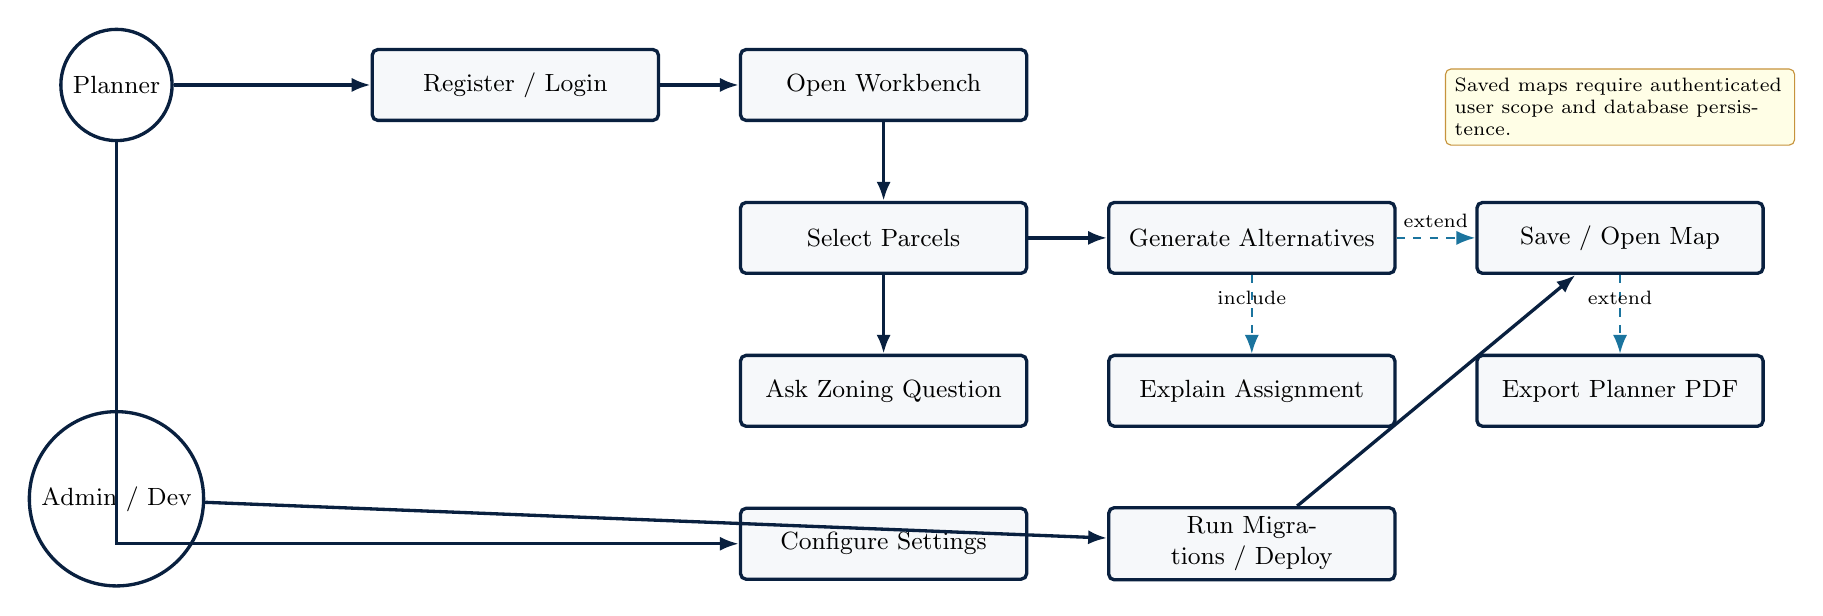
\begin{tikzpicture}[node distance=10mm]
\node[actor] (planner) {Planner};
\node[actor, below=34mm of planner] (admin) {Admin / Dev};
\node[block, right=25mm of planner] (auth) {Register / Login};
\node[block, right=of auth] (workbench) {Open Workbench};
\node[block, below=of workbench] (select) {Select Parcels};
\node[block, right=of select] (opt) {Generate Alternatives};
\node[block, below=of select] (zoning) {Ask Zoning Question};
\node[block, below=of opt] (explain) {Explain Assignment};
\node[block, right=of opt] (save) {Save / Open Map};
\node[block, right=of explain] (pdf) {Export Planner PDF};
\node[block, below=of zoning] (settings) {Configure Settings};
\node[block, right=of settings] (deploy) {Run Migrations / Deploy};
\draw[arrow] (planner) -- (auth);
\draw[arrow] (auth) -- (workbench);
\draw[arrow] (workbench) -- (select);
\draw[arrow] (select) -- (opt);
\draw[arrow] (select) -- (zoning);
\draw[dashedarrow] (opt) -- node[above,font=\scriptsize]{include} (explain);
\draw[dashedarrow] (opt) -- node[above,font=\scriptsize]{extend} (save);
\draw[dashedarrow] (save) -- node[above,font=\scriptsize]{extend} (pdf);
\draw[arrow] (planner) |- (settings);
\draw[arrow] (admin) -- (deploy);
\draw[arrow] (deploy) -- (save);
\node[note, above=7mm of save] {Saved maps require authenticated user scope and database persistence.};
\end{tikzpicture}}
\caption{GeoVision use case diagram}\label{fig:usecase}
\end{figure}

\section{Sequence Diagrams / System Sequence Diagram}
\sequencefour{Authentication system sequence diagram}{User}{React Auth Context}{FastAPI Auth Router}{PostgreSQL users}{submit credentials}{token and user session}
\sequencefour{Spatial optimization system sequence diagram}{Planner}{Environmental Page}{Spatial Optimizer API}{Redis / PostgreSQL}{selected parcels and settings}{plans, warnings, objectives}
\sequencefour{Saved map system sequence diagram}{Planner}{Plan Gallery}{Saved Map Router}{PostgreSQL saved\_maps}{save or open map}{saved map result}
\sequencefour{Copilot streaming system sequence diagram}{Planner}{Copilot Page}{Copilot Endpoint}{Tool Services}{planning query}{streamed events}

\section{Test Plan (Test Level, Testing Techniques)}
\begin{longtable}{p{0.20\textwidth}p{0.35\textwidth}p{0.35\textwidth}}
\caption{Test plan summary}\label{tab:testplan}\\
\toprule
Level & Focus & Example Test Areas \\
\midrule
Unit & Single functions and services. & config parsing, risk explainer, assignment explainer, spatial cache key, optimizer helpers. \\
Integration & API plus service boundaries. & auth endpoints, saved maps endpoints, spatial endpoints, RAG/explain endpoints. \\
System & End-to-end user workflows. & login to workbench, select parcels, optimize, save, open, explain, export. \\
Performance & Heavy operations. & optimization latency, cache hit/miss behavior, large selection handling. \\
Security & Access control and inputs. & user-scoped saved maps, token validation, API key guard, CORS settings. \\
\bottomrule
\end{longtable}

\section{Software Development Plan}
The development plan follows four FYP milestones: Midterm FYP-1 for foundation, Final FYP-1 for environmental and zoning workflows, Midterm FYP-2 for optimization and plan gallery, and Final FYP-2 for persistence, caching, reporting, and final stabilization.

\section{Wire-frames}
\begin{figure}[H]\centering
\resizebox{0.95\textwidth}{!}{%
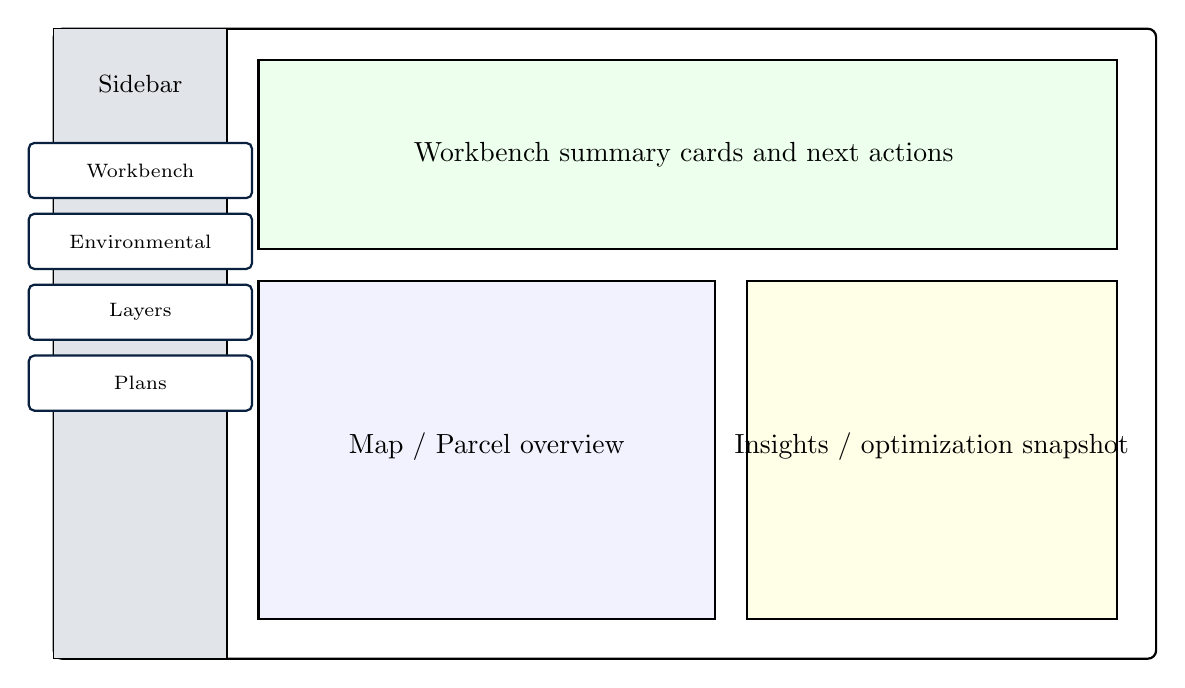
\begin{tikzpicture}
\draw[rounded corners=3pt, thick] (0,0) rectangle (14,8);
\draw[fill=gvblue!12] (0,0) rectangle (2.2,8);
\node[align=center,font=\small] at (1.1,7.3) {Sidebar};
\node[smallblock] at (1.1,6.2) {Workbench};
\node[smallblock] at (1.1,5.3) {Environmental};
\node[smallblock] at (1.1,4.4) {Layers};
\node[smallblock] at (1.1,3.5) {Plans};
\draw[fill=green!7, thick] (2.6,5.2) rectangle (13.5,7.6);
\node[align=center] at (8,6.4) {Workbench summary cards and next actions};
\draw[fill=blue!5, thick] (2.6,0.5) rectangle (8.4,4.8);
\node[align=center] at (5.5,2.7) {Map / Parcel overview};
\draw[fill=yellow!10, thick] (8.8,0.5) rectangle (13.5,4.8);
\node[align=center] at (11.15,2.7) {Insights / optimization snapshot};
\end{tikzpicture}}
\caption{Workbench wireframe}\end{figure}

\begin{figure}[H]\centering
\resizebox{0.95\textwidth}{!}{%
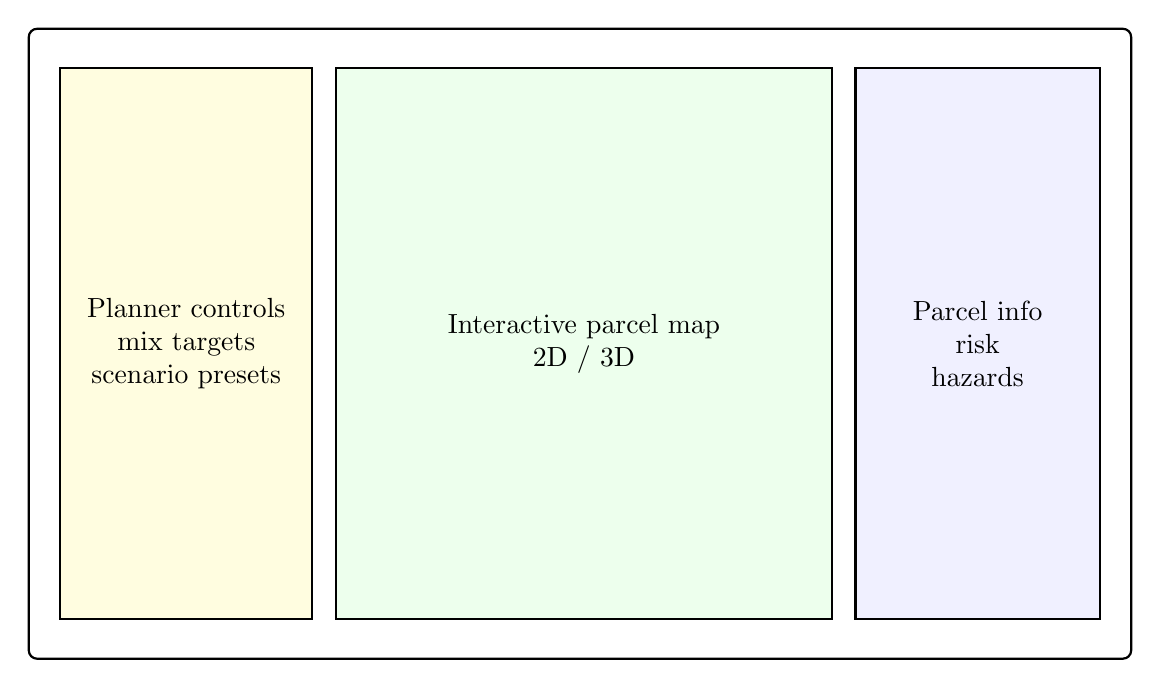
\begin{tikzpicture}
\draw[rounded corners=3pt, thick] (0,0) rectangle (14,8);
\draw[fill=yellow!12, thick] (0.4,0.5) rectangle (3.6,7.5);
\node[align=center] at (2,4) {Planner controls\\mix targets\\scenario presets};
\draw[fill=green!7, thick] (3.9,0.5) rectangle (10.2,7.5);
\node[align=center] at (7.05,4) {Interactive parcel map\\2D / 3D};
\draw[fill=blue!6, thick] (10.5,0.5) rectangle (13.6,7.5);
\node[align=center] at (12.05,4) {Parcel info\\risk\\hazards};
\end{tikzpicture}}
\caption{Environmental page wireframe}\end{figure}

\section{UI Screens}
The implemented UI surfaces are represented by the following logical screens rather than static screenshots: public welcome page, login page, registration page, protected main layout, workbench, environmental map, layers and zoning chat, plan gallery, saved plans panel, copilot, and settings. The exact visual appearance depends on frontend CSS, but the required screens and their responsibilities are documented in the user manual.

\chapter{Iteration Plan}
This chapter describes how the project proceeds through the four required FYP milestones.

\begin{longtable}{p{0.18\textwidth}p{0.26\textwidth}p{0.44\textwidth}}
\caption{Iteration plan by FYP milestone}\label{tab:iterationplan}\\
\toprule
Milestone & Main Theme & Planned / Implemented Modules \\
\midrule
Midterm FYP-1 & Foundation & project setup, authentication, database schema, basic frontend shell, map loading, configuration. \\
Final FYP-1 & Planning intelligence baseline & environmental risk view, zoning RAG, risk explanation, planner settings, map interaction. \\
Midterm FYP-2 & Optimization workflow & NSGA-II spatial optimization, plan gallery, objective display, assignment inspection. \\
Final FYP-2 & Persistence and polish & saved maps, Redis cache, workbench, assignment explanations, PDF export, Docker deployment, final testing. \\
\bottomrule
\end{longtable}

\flowfive{Overall iteration execution flow}{Foundation}{Environmental and zoning workflows}{Optimization and plan gallery}{Persistence and reporting}{Final verification}

\chapter{Iteration 1}
This iteration corresponds to Midterm FYP-1. Its theme is Foundation, authentication, database setup, and dashboard shell. The chapter follows the required artifact list from the provided FYP template.

\section{Architecture Diagram}

\begin{figure}[H]\centering
\includegraphics[width=0.98\textwidth]{architecture_diagram_fyp_1.png}
\caption{Iteration 1 architecture diagram}\end{figure}

\section{Use Case Diagram}

\begin{figure}[H]\centering
\includegraphics[width=0.88\textwidth]{usecase_diagram_fyp_1.png}
\caption{Iteration 1 use case diagram}\end{figure}

\section{Component Diagram}

\begin{figure}[H]\centering
\includegraphics[width=0.98\textwidth]{component_diagram_fyp_1.png}
\caption{Iteration 1 component diagram}\end{figure}

\section{Sequence Diagram}

\begin{figure}[H]\centering
\includegraphics[width=0.98\textwidth]{sequence_diagram_fyp_1.png}
\caption{Iteration 1 sequence diagram}\end{figure}

\section{Schema Design / ER Diagram}

The schema note for this iteration is: users only; saved\_maps planned for a later iteration.

\begin{figure}[H]\centering
\includegraphics[width=0.88\textwidth]{erd_fyp_1.png}
\caption{Iteration 1 schema design / ER diagram}\end{figure}

\section{Data Dictionary}

\begin{longtable}{p{0.22\textwidth}p{0.40\textwidth}p{0.28\textwidth}}
\caption{Iteration 1 data dictionary}\label{tab:iter6dict}\\
\toprule
Item & Important fields & Meaning \\
\midrule
\endfirsthead
\toprule
Item & Important fields & Meaning \\
\midrule
\endhead

User & id, email, username, hashed\_password, is\_active, created\_at, updated\_at & Persistent account record \\

Token & access\_token, token\_type, user & Authentication response \\

Settings & environment, database\_url, cors\_origins, jwt\_secret\_key & Runtime backend configuration \\

AuthContext & user, isAuthenticated, isLoading & Frontend session state \\

\bottomrule
\end{longtable}

\section{Data Structure Design}
The iteration uses the following data structures.
\begin{itemize}

\item \textbf{User}: Persistent account record. Important fields include id, email, username, hashed\_password, is\_active, created\_at, updated\_at.

\item \textbf{Token}: Authentication response. Important fields include access\_token, token\_type, user.

\item \textbf{Settings}: Runtime backend configuration. Important fields include environment, database\_url, cors\_origins, jwt\_secret\_key.

\item \textbf{AuthContext}: Frontend session state. Important fields include user, isAuthenticated, isLoading.

\end{itemize}

\section{Algorithm Design}
Register user: validate input, reject duplicates, hash password, insert user, sign JWT, return token and user payload. Login user: find account, verify password, sign JWT, return token. Protected route: read token, call current-user endpoint, render dashboard if valid, redirect otherwise.
\begin{enumerate}

\item Open public page.

\item Submit register or login form.

\item Validate credentials and hash/check password.

\item Issue bearer token.

\item Enter protected dashboard.

\end{enumerate}

\section{Development Phase}
Development in this iteration focused on modular code, explicit naming, and testable service boundaries. Backend code uses routers, schemas, services, utilities, and agent modules. Frontend code uses pages, components, contexts, hooks, and utility functions.

\subsection{Unit Test}
Relevant unit or focused tests include: test\_auth\_endpoints.py, test\_database.py, test\_config.py, test\_alembic\_users\_migration.py.

\subsection{Suites or Test Cases}
\begin{longtable}{p{0.28\textwidth}p{0.62\textwidth}}
\caption{Iteration 1 test cases}\\
\toprule
Test Case & Expected Result \\
\midrule

Valid workflow request & The main Authentication and Base Platform path returns successful output. \\

Invalid or missing input & The API or UI rejects the request and shows an error or fallback. \\
Persistence or state restoration & Stored state is restored only for the correct user or valid session. \\
Regression check & Existing tests continue passing after changes. \\
\bottomrule
\end{longtable}

\section{Maintainable Phase}
The maintainable phase ensures the iteration can be built, tested, deployed, and modified without breaking earlier workflows.

\subsection{CI / CD}
The expected CI pipeline installs backend dependencies, runs Pytest, checks frontend package installation, and can be extended with frontend build checks. Database migrations are run separately through Alembic or the Docker Compose migrate service.

\subsection{System-Level Test Suites, Test Cases}
System testing should run the user path from login to the relevant workflow output and verify that frontend state, backend response, and persistence/cache effects match expectations.

\subsection{SVN or GitHub (Optional)}
The project uses Git/GitHub-style source control. Feature work should be committed by module, merged through reviewed branches, and tagged at milestone submissions.

\subsection{Configuration / Setup and Tool Manual (Optional)}
For this iteration, setup focuses on Local backend, frontend development server, PostgreSQL configuration, Alembic users migration. The common commands are: install dependencies, configure environment variables, run migrations, start backend, start frontend, and run tests.

\chapter{Iteration 2}
This iteration corresponds to Final FYP-1. Its theme is Environmental analysis, map interaction, zoning RAG, and risk explanation. The chapter follows the required artifact list from the provided FYP template.

\section{Architecture Diagram}

\begin{figure}[H]\centering
\includegraphics[width=0.98\textwidth]{architecture_diagram_fyp_1.png}
\caption{Iteration 2 architecture diagram}\end{figure}

\section{Use Case Diagram}

\begin{figure}[H]\centering
\includegraphics[width=0.88\textwidth]{usecase_diagram_fyp_1.png}
\caption{Iteration 2 use case diagram}\end{figure}

\section{Component Diagram}

\begin{figure}[H]\centering
\includegraphics[width=0.98\textwidth]{component_diagram_fyp_1.png}
\caption{Iteration 2 component diagram}\end{figure}

\section{Sequence Diagram}

\begin{figure}[H]\centering
\includegraphics[width=0.98\textwidth]{sequence_diagram_fyp_1.png}
\caption{Iteration 2 sequence diagram}\end{figure}

\section{Schema Design / ER Diagram}

The schema note for this iteration is: users table remains active; zoning sessions are in memory through ChatSessionStore rather than a persistent table in this iteration.

\begin{figure}[H]\centering
\includegraphics[width=0.88\textwidth]{erd_fyp_1.png}
\caption{Iteration 2 schema design / ER diagram}\end{figure}

\section{Data Dictionary}

\begin{longtable}{p{0.22\textwidth}p{0.40\textwidth}p{0.28\textwidth}}
\caption{Iteration 2 data dictionary}\label{tab:iter7dict}\\
\toprule
Item & Important fields & Meaning \\
\midrule
\endfirsthead
\toprule
Item & Important fields & Meaning \\
\midrule
\endhead

GeoJSON Feature & geometry, properties, APN, hazard flags & Parcel input and display unit \\

Risk Contribution & factor, label, weight, active, contribution\_pct & Explanation of hazard score \\

Zoning Request & question, apn, context, session\_id & RAG chat input \\

Zoning Response & answer, session\_id, citations & RAG chat output \\

\bottomrule
\end{longtable}

\section{Data Structure Design}
The iteration uses the following data structures.
\begin{itemize}

\item \textbf{GeoJSON Feature}: Parcel input and display unit. Important fields include geometry, properties, APN, hazard flags.

\item \textbf{Risk Contribution}: Explanation of hazard score. Important fields include factor, label, weight, active, contribution\_pct.

\item \textbf{Zoning Request}: RAG chat input. Important fields include question, apn, context, session\_id.

\item \textbf{Zoning Response}: RAG chat output. Important fields include answer, session\_id, citations.

\end{itemize}

\section{Algorithm Design}
Risk explanation sums active hazard weights and sorts contributions. Counterfactual risk copies parcel properties, applies permitted hazard changes, recomputes the weighted score, and returns the delta. Zoning RAG builds a parcel-aware prompt, retrieves relevant regulation chunks when available, and returns a grounded answer or fallback response.
\begin{enumerate}

\item Load parcel GeoJSON.

\item Select parcel and read properties.

\item Compute/inspect environmental risk.

\item Send zoning question with APN context.

\item Display answer and citations/fallback.

\end{enumerate}

\section{Development Phase}
Development in this iteration focused on modular code, explicit naming, and testable service boundaries. Backend code uses routers, schemas, services, utilities, and agent modules. Frontend code uses pages, components, contexts, hooks, and utility functions.

\subsection{Unit Test}
Relevant unit or focused tests include: test\_rag\_and\_explain\_endpoints.py, test\_zoning\_rag\_service.py, test\_risk\_explainer.py, test\_suitability\_agent.py.

\subsection{Suites or Test Cases}
\begin{longtable}{p{0.28\textwidth}p{0.62\textwidth}}
\caption{Iteration 2 test cases}\\
\toprule
Test Case & Expected Result \\
\midrule

Valid workflow request & The main Environmental and Zoning Intelligence path returns successful output. \\

Invalid or missing input & The API or UI rejects the request and shows an error or fallback. \\
Persistence or state restoration & Stored state is restored only for the correct user or valid session. \\
Regression check & Existing tests continue passing after changes. \\
\bottomrule
\end{longtable}

\section{Maintainable Phase}
The maintainable phase ensures the iteration can be built, tested, deployed, and modified without breaking earlier workflows.

\subsection{CI / CD}
The expected CI pipeline installs backend dependencies, runs Pytest, checks frontend package installation, and can be extended with frontend build checks. Database migrations are run separately through Alembic or the Docker Compose migrate service.

\subsection{System-Level Test Suites, Test Cases}
System testing should run the user path from login to the relevant workflow output and verify that frontend state, backend response, and persistence/cache effects match expectations.

\subsection{SVN or GitHub (Optional)}
The project uses Git/GitHub-style source control. Feature work should be committed by module, merged through reviewed branches, and tagged at milestone submissions.

\subsection{Configuration / Setup and Tool Manual (Optional)}
For this iteration, setup focuses on Backend environment variables for RAG persistence, static frontend GeoJSON, and API base URL configuration. The common commands are: install dependencies, configure environment variables, run migrations, start backend, start frontend, and run tests.

\chapter{Iteration 3}
This iteration corresponds to Midterm FYP-2. Its theme is Spatial optimization, scenario presets, plan gallery, and assignment inspection. The chapter follows the required artifact list from the provided FYP template.

\section{Architecture Diagram}

\begin{figure}[H]\centering
\includegraphics[width=0.98\textwidth]{fypp_architecture_diagram.png}
\caption{Iteration 3 architecture diagram}\end{figure}

\section{Use Case Diagram}

\begin{figure}[H]\centering
\includegraphics[width=0.88\textwidth]{fypp-usecase.png}
\caption{Iteration 3 use case diagram}\end{figure}

\section{Component Diagram}

\begin{figure}[H]\centering
\includegraphics[width=0.98\textwidth]{fypp-component.png}
\caption{Iteration 3 component diagram}\end{figure}

\section{Sequence Diagram}

\begin{figure}[H]\centering
\includegraphics[width=0.98\textwidth]{fypp-sequence.png}
\caption{Iteration 3 sequence diagram}\end{figure}

\section{Schema Design / ER Diagram}

The schema note for this iteration is: saved\_maps table is introduced as a design target for storing optimization outputs in the next iteration.

\begin{figure}[H]\centering
\includegraphics[width=0.88\textwidth]{erd_fyp_1.png}
\caption{Iteration 3 schema design / ER diagram}\end{figure}

\section{Data Dictionary}

\begin{longtable}{p{0.22\textwidth}p{0.40\textwidth}p{0.28\textwidth}}
\caption{Iteration 3 data dictionary}\label{tab:iter8dict}\\
\toprule
Item & Important fields & Meaning \\
\midrule
\endfirsthead
\toprule
Item & Important fields & Meaning \\
\midrule
\endhead

SpatialOptimizeRequest & parcels, target\_mix, num\_output\_plans, population\_size, generations & Optimization input \\

SpatialOptimizationPlan & rank, crowding\_distance, objectives, assignments & Generated alternative \\

Assignment & parcel\_id, use\_code, use\_label & Parcel-level land-use output \\

Workspace Metadata & duration, plan count, selected count, warnings & Latest optimization summary \\

\bottomrule
\end{longtable}

\section{Data Structure Design}
The iteration uses the following data structures.
\begin{itemize}

\item \textbf{SpatialOptimizeRequest}: Optimization input. Important fields include parcels, target\_mix, num\_output\_plans, population\_size, generations.

\item \textbf{SpatialOptimizationPlan}: Generated alternative. Important fields include rank, crowding\_distance, objectives, assignments.

\item \textbf{Assignment}: Parcel-level land-use output. Important fields include parcel\_id, use\_code, use\_label.

\item \textbf{Workspace Metadata}: Latest optimization summary. Important fields include duration, plan count, selected count, warnings.

\end{itemize}

\section{Algorithm Design}
The optimization workflow converts selected GeoJSON features into parcel records, normalizes target mix, builds optional adjacency relationships, initializes a population, evaluates objective functions, performs non-dominated sorting and crowding-distance selection, and returns top candidate plans with assignments.
\begin{enumerate}

\item Select parcels.

\item Apply scenario preset or mix target.

\item Submit optimization payload.

\item Run optimizer and rank plans.

\item Inspect candidate plans.

\end{enumerate}

\section{Development Phase}
Development in this iteration focused on modular code, explicit naming, and testable service boundaries. Backend code uses routers, schemas, services, utilities, and agent modules. Frontend code uses pages, components, contexts, hooks, and utility functions.

\subsection{Unit Test}
Relevant unit or focused tests include: test\_spatial\_endpoints.py, test\_spatial\_agent.py, test\_nsga2.py, test\_optimizer.py, test\_objectives.py.

\subsection{Suites or Test Cases}
\begin{longtable}{p{0.28\textwidth}p{0.62\textwidth}}
\caption{Iteration 3 test cases}\\
\toprule
Test Case & Expected Result \\
\midrule

Valid workflow request & The main Spatial Optimization and Plan Gallery path returns successful output. \\

Invalid or missing input & The API or UI rejects the request and shows an error or fallback. \\
Persistence or state restoration & Stored state is restored only for the correct user or valid session. \\
Regression check & Existing tests continue passing after changes. \\
\bottomrule
\end{longtable}

\section{Maintainable Phase}
The maintainable phase ensures the iteration can be built, tested, deployed, and modified without breaking earlier workflows.

\subsection{CI / CD}
The expected CI pipeline installs backend dependencies, runs Pytest, checks frontend package installation, and can be extended with frontend build checks. Database migrations are run separately through Alembic or the Docker Compose migrate service.

\subsection{System-Level Test Suites, Test Cases}
System testing should run the user path from login to the relevant workflow output and verify that frontend state, backend response, and persistence/cache effects match expectations.

\subsection{SVN or GitHub (Optional)}
The project uses Git/GitHub-style source control. Feature work should be committed by module, merged through reviewed branches, and tagged at milestone submissions.

\subsection{Configuration / Setup and Tool Manual (Optional)}
For this iteration, setup focuses on Spatial endpoint runs inside FastAPI; frontend sends payload from environmental page and stores plans in shared workspace state. The common commands are: install dependencies, configure environment variables, run migrations, start backend, start frontend, and run tests.

\chapter{Iteration 4}
This iteration corresponds to Final FYP-2. Its theme is Workbench, saved maps, Redis cache, assignment explanation, PDF export, and deployment. The chapter follows the required artifact list from the provided FYP template.

\section{Architecture Diagram}

\begin{figure}[H]\centering
\includegraphics[width=0.98\textwidth]{architecture_diagram_final.png}
\caption{Iteration 4 architecture diagram}\end{figure}

\section{Use Case Diagram}

\begin{figure}[H]\centering
\includegraphics[width=0.88\textwidth]{final-Usecase.png}
\caption{Iteration 4 use case diagram}\end{figure}

\section{Component Diagram}

\begin{figure}[H]\centering
\includegraphics[width=0.98\textwidth]{final-Component.png}
\caption{Iteration 4 component diagram}\end{figure}

\section{Sequence Diagram}

\begin{figure}[H]\centering
\includegraphics[width=0.98\textwidth]{final-sequence.png}
\caption{Iteration 4 sequence diagram}\end{figure}

\section{Schema Design / ER Diagram}

The schema note for this iteration is: users has one-to-many saved\_maps with on-delete cascade; saved\_maps stores parcel and optimization JSONB payloads.

\begin{figure}[H]\centering
\includegraphics[width=0.75\textwidth,height=0.55\textheight,keepaspectratio]{final-ERD.png}
\caption{Iteration 4 schema design / ER diagram}\end{figure}

\section{Data Dictionary}

\begin{longtable}{p{0.22\textwidth}p{0.40\textwidth}p{0.28\textwidth}}
\caption{Iteration 4 data dictionary}\label{tab:iter9dict}\\
\toprule
Item & Important fields & Meaning \\
\midrule
\endfirsthead
\toprule
Item & Important fields & Meaning \\
\midrule
\endhead

SavedMap & id, user\_id, name, description, parcel\_count, plan\_count, selected\_plan\_rank, input\_parcels, optimization\_result & Persistent map record \\

Cache Key & normalized features and optimization settings hash & Redis optimization cache lookup \\

Assignment Explanation & headline, reasons, warnings, scores, risk\_level & Planner-friendly explanation output \\

Planner Report & summary, objective table, warnings, map image, appendix & Exported PDF document \\

\bottomrule
\end{longtable}

\section{Data Structure Design}
The iteration uses the following data structures.
\begin{itemize}

\item \textbf{SavedMap}: Persistent map record. Important fields include id, user\_id, name, description, parcel\_count, plan\_count, selected\_plan\_rank, input\_parcels, optimization\_result.

\item \textbf{Cache Key}: Redis optimization cache lookup. Important fields include normalized features and optimization settings hash.

\item \textbf{Assignment Explanation}: Planner-friendly explanation output. Important fields include headline, reasons, warnings, scores, risk\_level.

\item \textbf{Planner Report}: Exported PDF document. Important fields include summary, objective table, warnings, map image, appendix.

\end{itemize}

\section{Algorithm Design}
The final integration computes canonical cache keys for optimization payloads, stores and reads JSON from Redis when available, persists saved maps to PostgreSQL under the authenticated user ID, explains assignments with suitability/risk/zoning/target logic, and builds a planner PDF from selected plan state and captured map image where available.
\begin{enumerate}

\item Generate or open plan.

\item Explain selected assignment.

\item Save optimization result.

\item Reload saved map when needed.

\item Export planner PDF report.

\end{enumerate}

\section{Development Phase}
Development in this iteration focused on modular code, explicit naming, and testable service boundaries. Backend code uses routers, schemas, services, utilities, and agent modules. Frontend code uses pages, components, contexts, hooks, and utility functions.

\subsection{Unit Test}
Relevant unit or focused tests include: test\_saved\_maps\_endpoints.py, test\_assignment\_explainer.py, test\_spatial\_cache.py, test\_copilot\_endpoint.py, test\_orchestrator\_endpoints.py, check-plan-gallery-assignment-explanations.mjs.

\subsection{Suites or Test Cases}
\begin{longtable}{p{0.28\textwidth}p{0.62\textwidth}}
\caption{Iteration 4 test cases}\\
\toprule
Test Case & Expected Result \\
\midrule

Valid workflow request & The main Persistence, Reporting, and Final Integration path returns successful output. \\

Invalid or missing input & The API or UI rejects the request and shows an error or fallback. \\
Persistence or state restoration & Stored state is restored only for the correct user or valid session. \\
Regression check & Existing tests continue passing after changes. \\
\bottomrule
\end{longtable}

\section{Maintainable Phase}
The maintainable phase ensures the iteration can be built, tested, deployed, and modified without breaking earlier workflows.

\subsection{CI / CD}
The CI pipeline installs backend dependencies, runs Pytest, and checks the frontend build. On merge to main, Vercel automatically rebuilds and redeploys the frontend. The Hugging Face Space rebuilds automatically from the repository. Database migrations are run once against Neon by executing \code{alembic upgrade head} with the production \code{DATABASE\_URL}.

\subsection{System-Level Test Suites, Test Cases}
System testing should run the user path from login to the relevant workflow output and verify that frontend state, backend response, and persistence/cache effects match expectations.

\subsection{SVN or GitHub (Optional)}
The project uses Git/GitHub-style source control. Feature work should be committed by module, merged through reviewed branches, and tagged at milestone submissions.

\subsection{Configuration / Setup and Tool Manual (Optional)}
For production, the frontend is deployed to Vercel (connect GitHub repository, set \code{VITE\_API\_URL} to the Hugging Face Spaces URL). The backend is deployed to Hugging Face Spaces as a Docker Space with \code{DATABASE\_URL} set as a repository secret pointing to the Neon cloud PostgreSQL instance. Alembic migrations are run once against Neon using \code{alembic upgrade head} before the Space starts. For local development, Docker Compose provides the same services locally. The common commands are: configure \code{.env} with Neon \code{DATABASE\_URL}, run \code{alembic upgrade head}, start backend, start frontend, and run tests.

\chapter{Implementation Details}
This chapter provides the procedural and algorithmic details that are not fully covered by the design diagrams. The focus is on how the implemented backend and frontend workflows cooperate.

\section{Authentication Procedure}
Authentication is implemented through a typical token-based flow. The user submits credentials to the backend. During registration, the backend validates uniqueness, hashes the password, stores the user, and returns a JWT access token. During login, the backend verifies the password and signs a token containing the user identifier. Protected frontend routes read the token from browser storage and validate the current user before rendering the dashboard.

\section{Planner Workspace State}
The frontend separates long-lived planner state into contexts. Authentication state is handled by the authentication context. Runtime planner settings are handled by the planner settings context and persisted in local storage. Parcel selections, loaded parcel features, primary selected parcel, generated plans, objective names, active plan index, and latest optimization metadata are handled by the planner workspace context. This separation avoids passing large state objects manually between pages.

\section{Environmental Risk Explanation}
The risk explainer uses a transparent weighted-score procedure. Each hazard flag has a fixed weight. If the flag is active, its weight contributes to the score; otherwise, it contributes zero. Contributions are sorted from highest to lowest and returned with labels such as floodplain, fault zone, liquefaction, steep slope, fire hazard, ESA, and MSCP habitat.

\flowfive{Risk explanation procedure}{Read parcel properties}{Check hazard flags}{Apply configured weights}{Sort contribution list}{Return total and breakdown}

\section{Counterfactual Risk Procedure}
Counterfactual risk analysis copies the original parcel properties, applies user-provided hazard changes, recalculates the weighted score, and returns the original score, counterfactual score, delta, and list of applied changes. This makes the feature explainable because the user can see exactly which flags changed the result.

\section{Zoning RAG Procedure}
The zoning RAG workflow accepts a natural-language question, optional APN, optional parcel context, and session identifier. The backend uses the RAG service when available to retrieve relevant zoning information and generate an answer. If retrieval infrastructure is unavailable, the endpoint can still return controlled fallback behavior rather than crashing the whole application.

\sequencefour{Zoning RAG procedural sequence}{Planner}{ZoningChatPanel}{RAG Endpoint}{RAG Service / Store}{question and parcel context}{answer with session state}

\section{Spatial Optimization Procedure}
Spatial optimization receives selected parcel GeoJSON features and planner settings. The backend extracts parcel records, validates geometry, normalizes target land-use mix, builds optional adjacency relationships, configures the optimizer, and executes the multi-objective search. Candidate plans are returned with rank, objective values, crowding distance, and parcel assignments.

\begin{figure}[H]\centering
\resizebox{0.95\textwidth}{!}{%
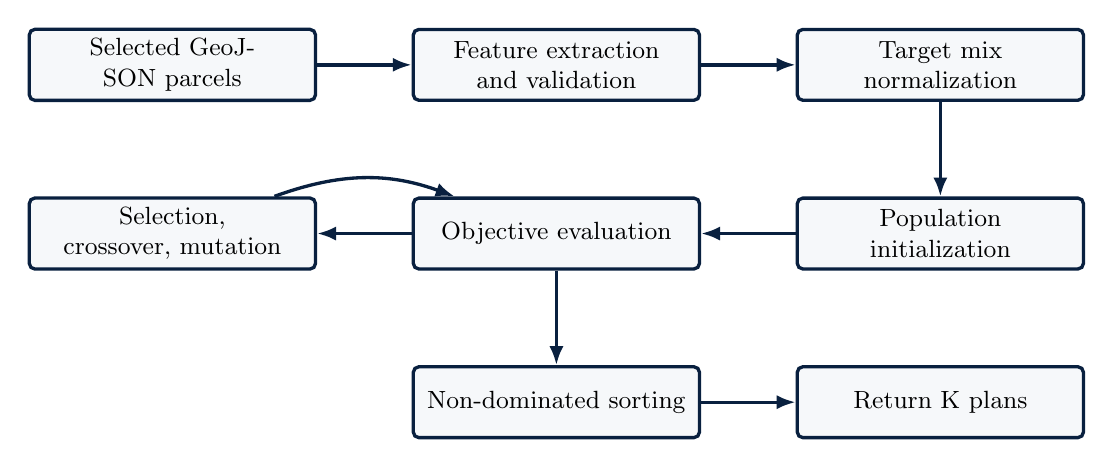
\begin{tikzpicture}[node distance=12mm]
\node[block] (a) {Selected GeoJSON parcels};
\node[block, right=of a] (b) {Feature extraction and validation};
\node[block, right=of b] (c) {Target mix normalization};
\node[block, below=of c] (d) {Population initialization};
\node[block, left=of d] (e) {Objective evaluation};
\node[block, left=of e] (f) {Selection, crossover, mutation};
\node[block, below=of e] (g) {Non-dominated sorting};
\node[block, right=of g] (h) {Return K plans};
\draw[arrow] (a)--(b);\draw[arrow] (b)--(c);\draw[arrow] (c)--(d);\draw[arrow] (d)--(e);\draw[arrow] (e)--(f);\draw[arrow] (f) to[bend left=20] (e);\draw[arrow] (e)--(g);\draw[arrow] (g)--(h);
\end{tikzpicture}}
\caption{Spatial optimization implementation procedure}
\end{figure}

\section{Redis Spatial Cache Procedure}
The optimization cache builds a canonical JSON payload from sorted parcel features and optimization settings. The payload includes cache version, number of output plans, population size, generations, adjacency settings, and normalized target mix. A SHA-256 digest becomes the cache key. If Redis is configured and reachable, repeated equivalent optimization requests can reuse stored JSON output. If Redis is unavailable, the backend falls back to normal processing.

\section{Saved Maps Procedure}
Saved maps are user-scoped. A create request stores the name, description, selected plan rank, input parcel list, and full optimization result. The service calculates parcel count and plan count from the payload. List requests return metadata-only records. Open requests return the full saved payload. Delete requests remove only records owned by the authenticated user.

\section{Assignment Explanation Procedure}
The assignment explainer compares assigned use with suitability scores, best suitability use, environmental risk, active hazard labels, zoning signals, and target mix. The procedure avoids repeating the same generic reason for every parcel. It adds reasons when the assigned use is suitable or policy-supported and warnings when risk, hazards, or low suitability require planner review.

\section{Planner PDF Export Procedure}
The plan gallery export builds a browser-side PDF report. The report includes plan summary, target mix versus actual mix, objective values, warnings, conflicts, selected plan explanation, assignment samples, assumptions, and appendix notes. Where the frontend can capture the map element, the report includes a plan image to make the PDF look closer to real land-use planning reports.

\section{Configuration and Deployment Procedure}
The production deployment uses three cloud services: Vercel hosts the compiled React frontend as a global CDN-distributed static application; Hugging Face Spaces hosts the FastAPI backend inside a Docker container; and Neon provides cloud-hosted PostgreSQL accessible over SSL. The backend reads \code{DATABASE\_URL} from a Hugging Face repository secret and connects to Neon on startup. Alembic migrations are executed once against Neon before the Space is made public. Redis is optional and gracefully absent in the free-tier Hugging Face environment. For local development, Docker Compose replicates the same topology with local containers.

\chapter{User Manual}
\section{Starting the System}
The production system is cloud-hosted. Open the Vercel URL in a browser to access the React frontend. The frontend communicates with the FastAPI backend hosted on Hugging Face Spaces, and data is persisted in Neon cloud PostgreSQL. No local installation is required to use the deployed system.

For local development, configure \code{.env} with the \code{DATABASE\_URL} pointing to Neon (or a local PostgreSQL instance), run \code{alembic upgrade head} once to create the schema, then start the backend with \code{uvicorn main:app} and the frontend with \code{npm run dev}.

\section{Registering and Logging In}
\begin{enumerate}
  \item Open the welcome page.
  \item Choose register if no account exists.
  \item Enter username, email, and password.
  \item After successful registration or login, the application opens the protected dashboard.
\end{enumerate}

\section{Using the Workbench}
The workbench is the planner command center. It summarizes loaded parcels, selected parcels, selected area, average risk, generated plans, and next actions. Use it to move quickly to the environmental page, layers page, plan gallery, or plan generation workflow.

\section{Selecting Parcels}
Open the environmental page and use the map to select parcels. The system supports individual selection, bulk selection, clearing selection, and selecting all loaded parcels. The selected parcel IDs and feature objects are shared with other planning workflows.

\section{Generating Alternatives}
\begin{enumerate}
  \item Select one or more parcels.
  \item Adjust target mix values for residential, commercial, industrial, and green use.
  \item Optionally apply a scenario preset.
  \item Choose number of output plans and optimizer settings.
  \item Run the optimizer.
  \item Open the plan gallery to compare alternatives.
\end{enumerate}

\section{Reviewing Plans}
The plan gallery shows generated alternatives, objective values, assignments, warnings, and plan comparison information. Select a plan to inspect parcel-level assignment details. Click a parcel to request an assignment explanation when available.

\section{Saving and Opening Maps}
After generating a plan, use the save option to store the optimization result in the database. Saved maps can be listed, opened, and deleted from the saved plans panel. Opening a saved map restores input parcels and generated plan results into the workspace.

\section{Asking Zoning Questions}
Open the layers page, select a parcel, and ask a zoning question. The system sends the question together with parcel context to the zoning RAG endpoint. Answers may include citations or fallback text depending on the available retrieval setup.

\section{Using the Copilot}
Open the copilot page and enter a planning question. The copilot streams intermediate events such as agent start, agent completion, text chunks, final response, or error events. This makes the workflow more inspectable than a single opaque response.

\section{Exporting the Planner PDF}
Open the plan gallery, select a plan, and choose the planner PDF export action. The report is generated in the browser and includes summaries, objective information, warnings, explanations, and a map image when the frontend can capture it.

\section{Changing Settings}
Open the settings page to adjust scenario generation, regulatory guidance, environmental thresholds, user account display data, and plan-alternative limits. Settings are stored in browser local storage.

\chapter{Conclusions and Future Work}
\section{Conclusion}
GeoVision demonstrates a full-stack, AI-assisted GIS planning platform that follows a planner-centered workflow. The implemented system combines authentication, workbench summaries, environmental map interaction, zoning RAG, spatial optimization, assignment explanation, saved maps, Redis caching, copilot streaming, and planner PDF export. The most important result is not a single model or endpoint, but the integration of several planning-support capabilities into one inspectable dashboard.

This report follows the provided FYP requirements structure and includes the required design artifacts across four iterations: domain/class diagrams, component diagrams, layer diagrams, structure charts, flow diagrams, DFDs, data dictionaries, activity diagrams, state machines, sequence diagrams, interaction overview diagrams, ER diagrams, data structure designs, algorithm descriptions, testing sections, CI/CD notes, deployment diagrams, GitHub notes, and setup guidance.

\section{Future Work}
Future improvements include live GIS ingestion, stronger zoning citation verification, collaborative review workflows, user roles and admin dashboards, plan approval states, richer report templates, spatial database support through PostGIS, better map image capture during PDF export, background optimization jobs for large areas, and more rigorous validation with real planners.

\begin{thebibliography}{5}

\bibitem{mai2025geoai}
G.~Mai, Y.~Hu, S.~Gao, R.~Cao, V.~Herfort, Y.~Xu, and A.~Zipf,
``Towards the next generation of Geospatial Artificial Intelligence,''
\textit{International Journal of Geographical Information Science}, 2025.

\bibitem{geojson2016}
H.~Butler, M.~Daly, A.~Doyle, S.~Gillies, S.~Hagen, and T.~Schaub,
``The GeoJSON Format,''
IETF RFC~7946, August 2016.

\bibitem{lewis2020rag}
P.~Lewis, E.~Perez, A.~Piktus, F.~Petroni, V.~Karpukhin, N.~Goyal, H.~K\"{u}ttler, M.~Lewis, W.~Yih, T.~Rockt\"{a}schel, S.~Riedel, and D.~Kiela,
``Retrieval-Augmented Generation for Knowledge-Intensive NLP Tasks,''
in \textit{Advances in Neural Information Processing Systems (NeurIPS)}, vol.~33, 2020.

\bibitem{deb2002nsga}
K.~Deb, A.~Pratap, S.~Agarwal, and T.~Meyarivan,
``A fast and elitist multiobjective genetic algorithm: NSGA-II,''
\textit{IEEE Transactions on Evolutionary Computation}, vol.~6, no.~2, pp.~182--197, 2002.

\bibitem{luan2024landuse}
C.~Luan, Y.~Liu, Z.~Li, Y.~Liang, and Y.~Liu,
``Multi-objective land use optimization based on integrated NSGA-II--PLUS model: Comprehensive consideration of economic development and ecosystem services value enhancement,''
\textit{Journal of Cleaner Production}, vol.~434, 2024.

\end{thebibliography}

\end{document}
